\documentclass{memoir} 
\usepackage{graphicx}
\usepackage{tikz}
\newsubfloat{figure}

\begin{document}

\begin{figure}[htbp]
\centering
\subbottom[Convex set]{
    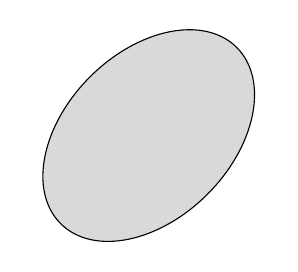
\begin{tikzpicture}
    \draw[rotate=-45,fill=gray!30] (0,0) ellipse (30pt and 45pt);
    %\draw (current bounding box.south east) rectangle (current bounding box.north west);
    \end{tikzpicture}
}
\hspace{1cm}
\subbottom[Non-convex set]{
    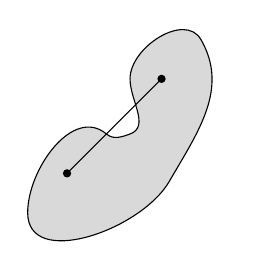
\begin{tikzpicture}
    \useasboundingbox (-1,-1.35) rectangle (1.5,1.35); % values found by trial and error
    \draw[fill=gray!30] (0,0) to [out=140,in=90] (-1,-1)
    to [out=-90,in=240] (0.8,-0.6)
    to [out=60,in=-60] (1.2,1.2)
    to [out=120,in=90] (0.3,0.7)
    to [out=-90,in=20] (0.3,0)
    to [out=200,in=-40] (0,0);
    \draw (-0.5,-0.5) -- (0.7,0.7);
    \fill (-0.5,-0.5) circle[radius=1.5pt];
    \fill (0.7,0.7) circle[radius=1.5pt];
    %\draw (current bounding box.south east) rectangle (current bounding box.north west);
    \end{tikzpicture}
}
\caption{Graphical interpretation of convex sets.}
\label{fig:convexSet}
\end{figure}
%https://tex.stackexchange.com/questions/302589/alignment-of-tikz-pictures-in-subfigures/302604#302604


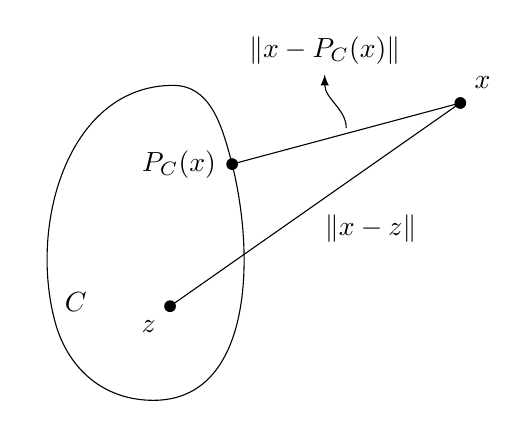
\begin{tikzpicture}[bullet/.style={circle,fill,inner sep=1.5pt,node contents={}}]
 \draw (0,0) node[bullet,label=left:$P_C(x)$,alias=PC]  -- (15:3) coordinate[midway] (aux)
    node[bullet,label=above right:$x$] -- ++ (-145:4.5) node[midway,below right]{$\|x-z\|$}     node[bullet,label=below left:$z$];
 \draw (PC) to[out=105,in=0] ++ (-0.75,1) to[out=180,in=105] ++ (-1.5,-3)
 node[above right]{$C$} to[out=-75,in=180] ++ (1.25,-1) to[out=0,in=-75] cycle;
 \draw[shorten <=2pt,-latex] (aux) to[out=90,in=-90] ++ (110:0.8) node[above]{$\|x-P_C(x)\|$};
\end{tikzpicture}
%https://tex.stackexchange.com/questions/497589/drawing-a-projection-on-closed-convex-with-tikz




\end{document}